Question principale:\\
Compte tenu de l'augmentation constante et rapide des annotations automatiques, un système expert peut il détecter les annotations inconsistantes et informer les possibles annotations manquantes vis à vis d'un organisme prokaryotes? 

idée directrices:
l'inférence logiques des prédictions peut se faire via une représentation en graphes des connaissances et l'utilisation de la logique non classiques permettant de représenter l'inconnu et la contradiction.

histoires:

herbs
   représentation en dag des connaissances
   description manuel des connaissances
   and or graph 
   logique classique T / F
   prédiction et expectation
   conclusion
   
Mais descriptions des connaissances fastidieuses .…… 
les prédictions inconnu sont considéré absentes suivant le principe du tiers exclut
ne peut pas gérer la contradictions..
structurations de l'information sous forme de phrases

vers une représentation des connaissances orienté-objets
vers une logique à 4 valeurs T,F,B,N pour gérer l'inconnu et la contradiction

belnap et ses tables de vérité

oui mais certains résultat semble incohérent  N ou B donc T ...

vers une représentation ensemblistes des connaissances et de leur valeurs de vérité
  - les ensembles et leur représentation en graphe conceptuelle
  - les valeurs de vérité généralisés

\begin{refsegment}
\chapter{GROOLS}
\section{Le début de GROOLS}
expliqué les ratés
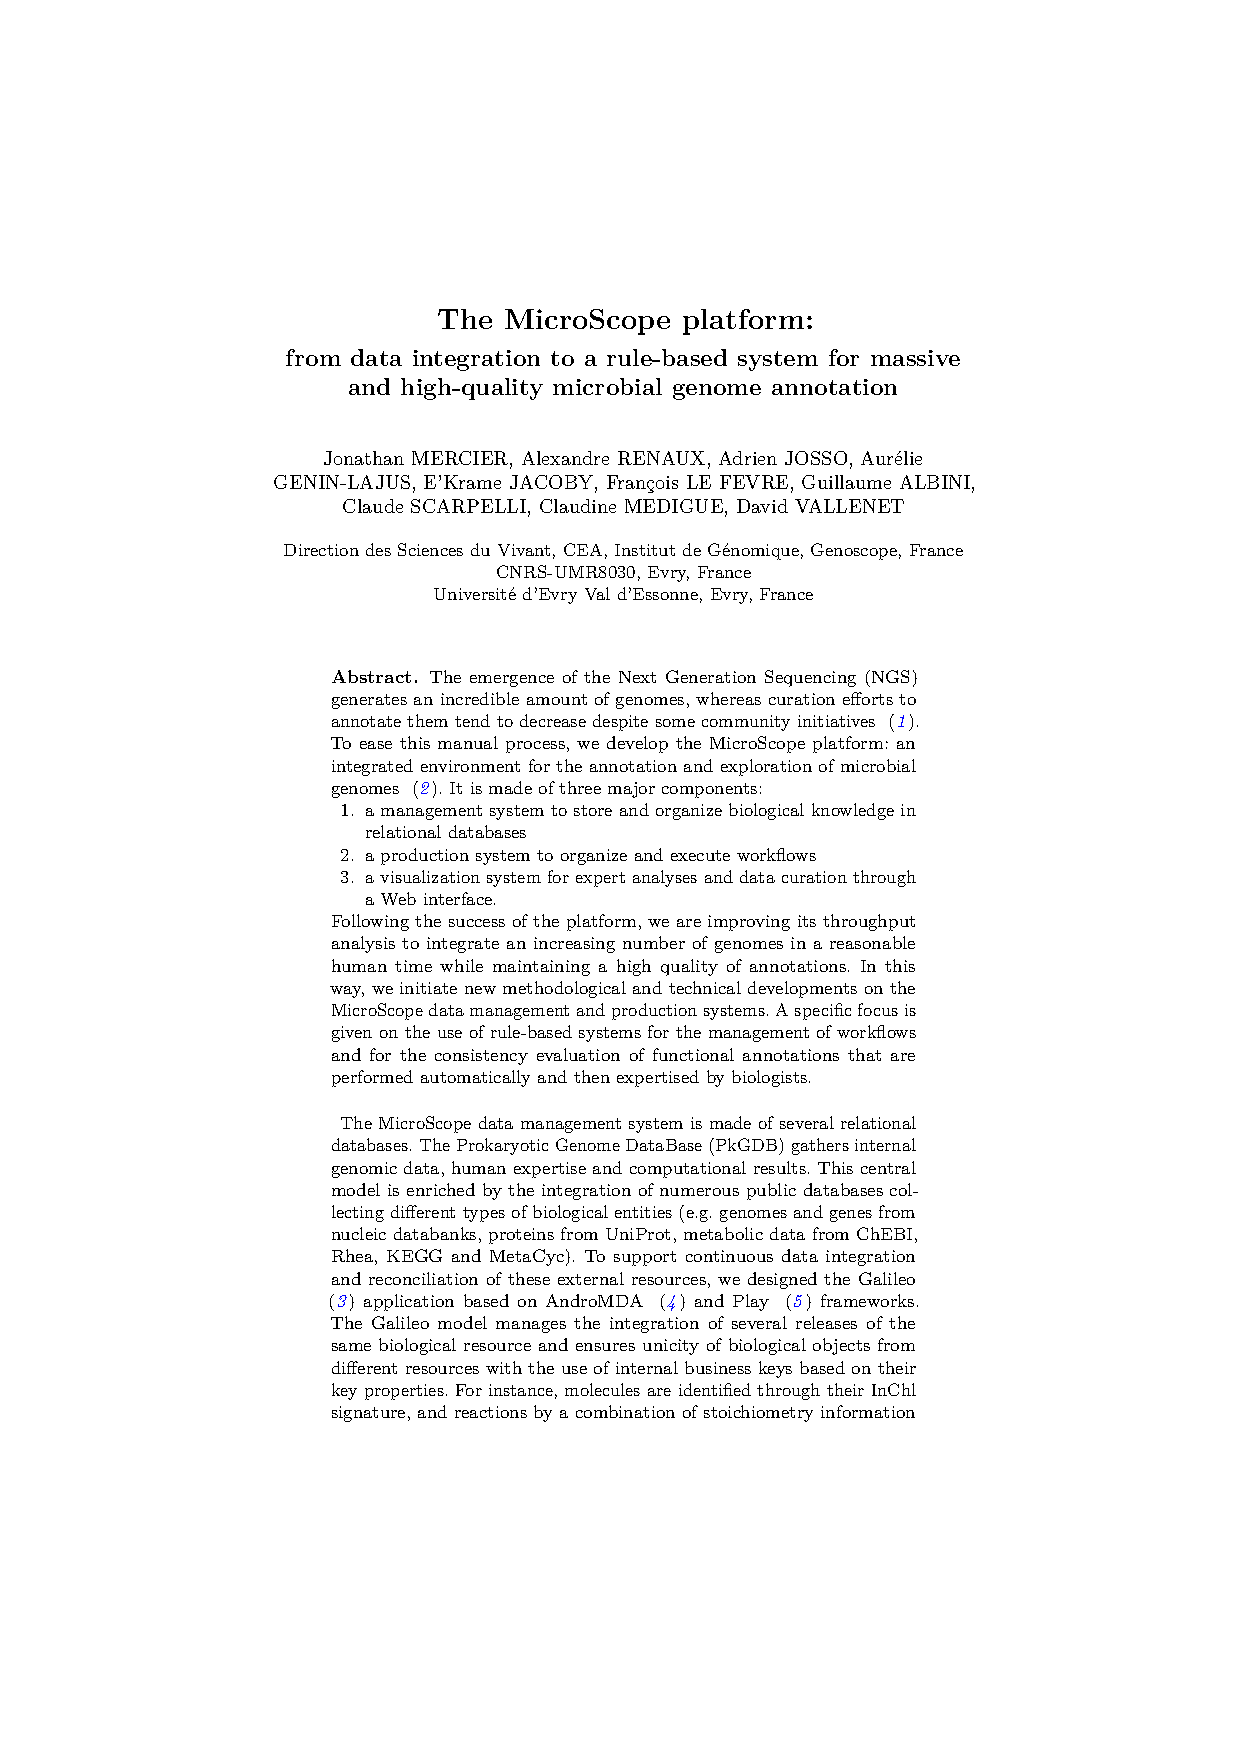
\includepdf[pages=-]{img/DILS_2014.pdf}

\begin{shadedfigure}
    \centering
    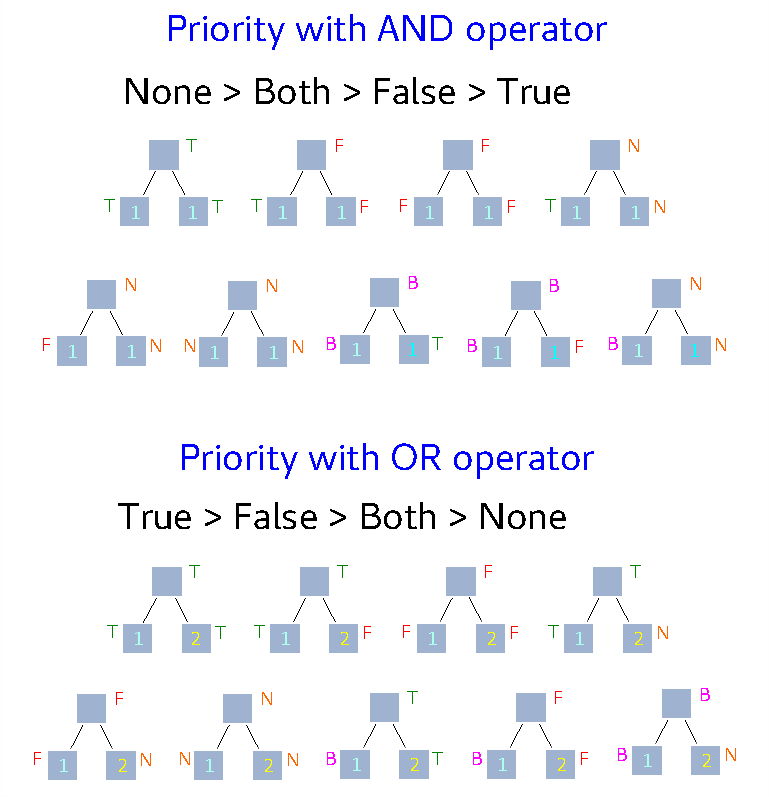
\includegraphics[width=\textwidth]{img/four_values_priorities_rules.pdf}
    \caption{  }
    \label{fig:seven_truth_values}
\end{shadedfigure}

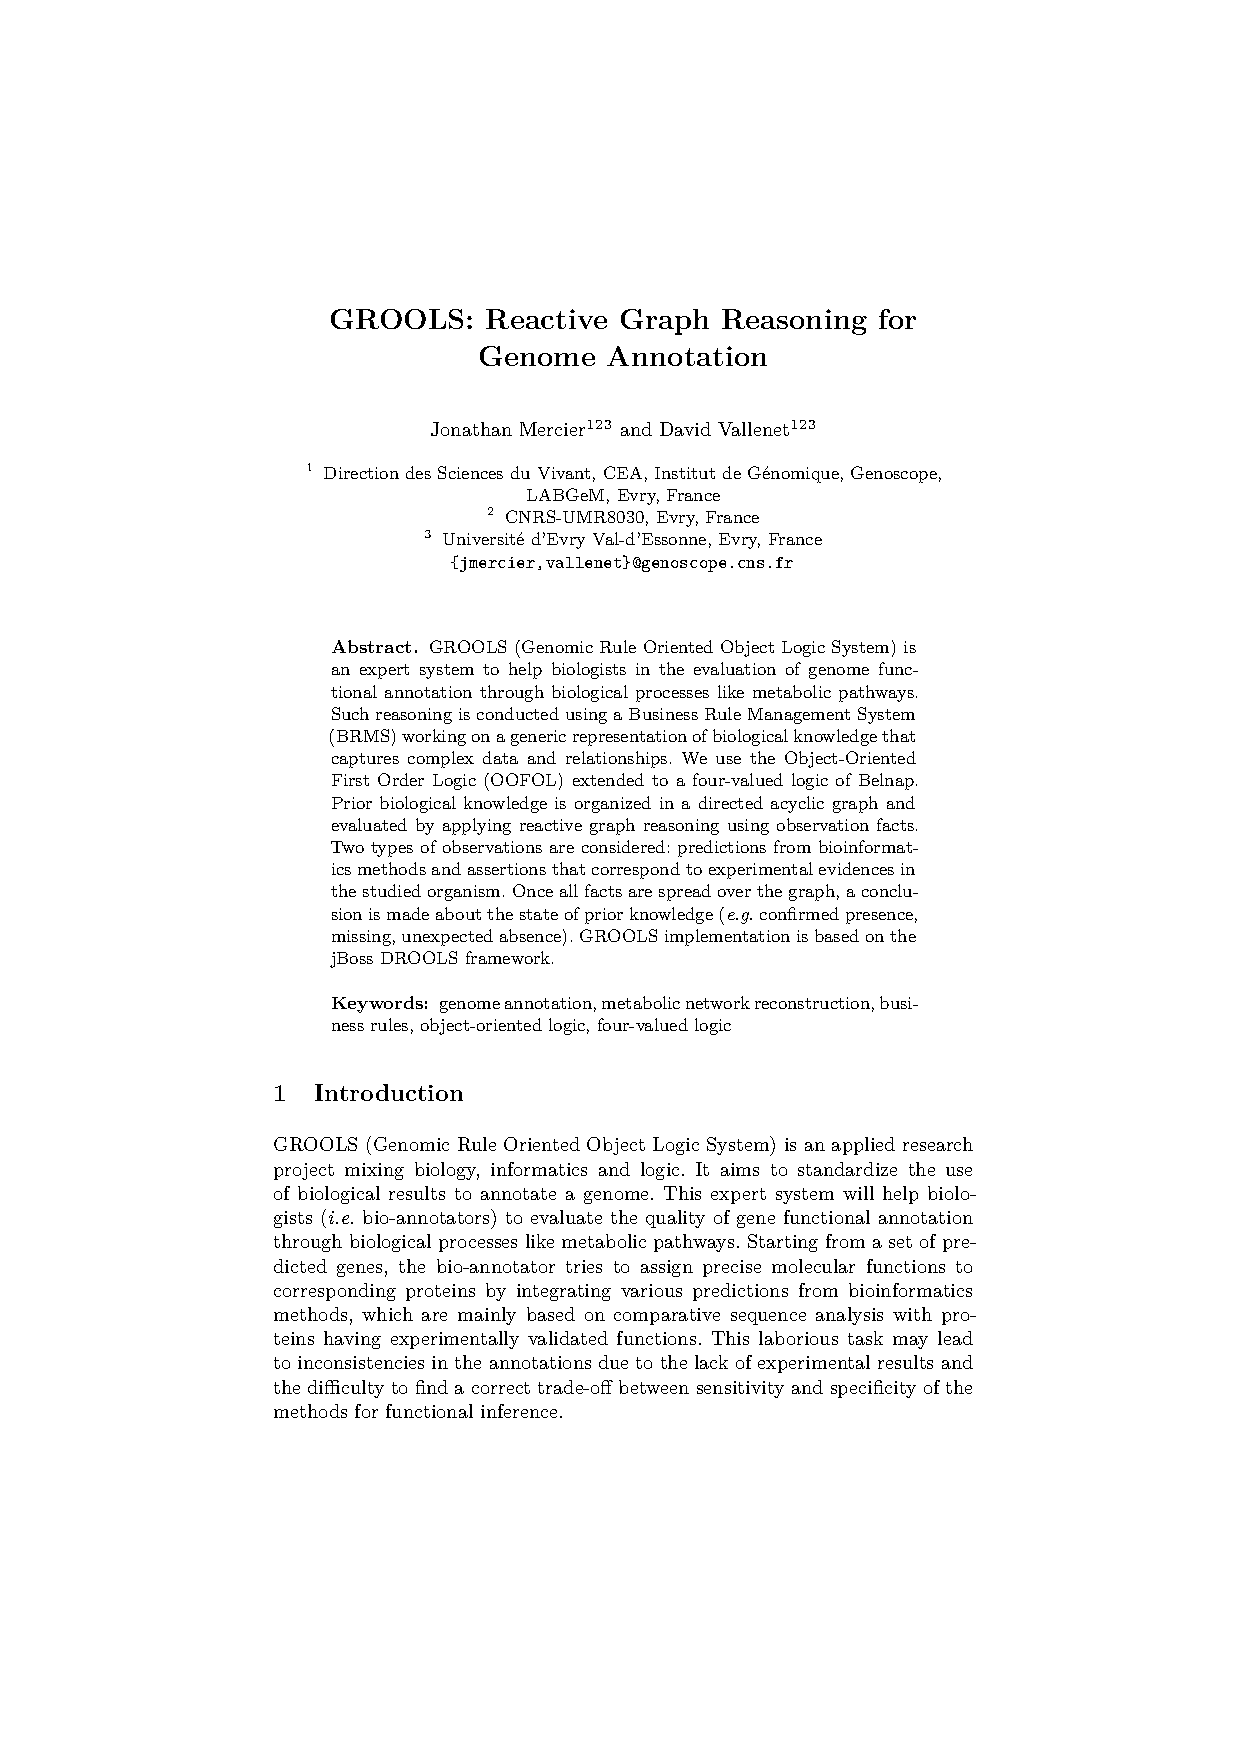
\includepdf[pages=-]{img/GROOLS__Reactive_Graph_Reasoning_for_Genome_Annotation.pdf}

7 valeurs de vérité mais pas encore l'utilisation de l'ensemble vide


\section{Vers un raisonnement descriptif}
ensembliste valeur de vérité généralisé



\begin{shadedfigure}
    \centering
    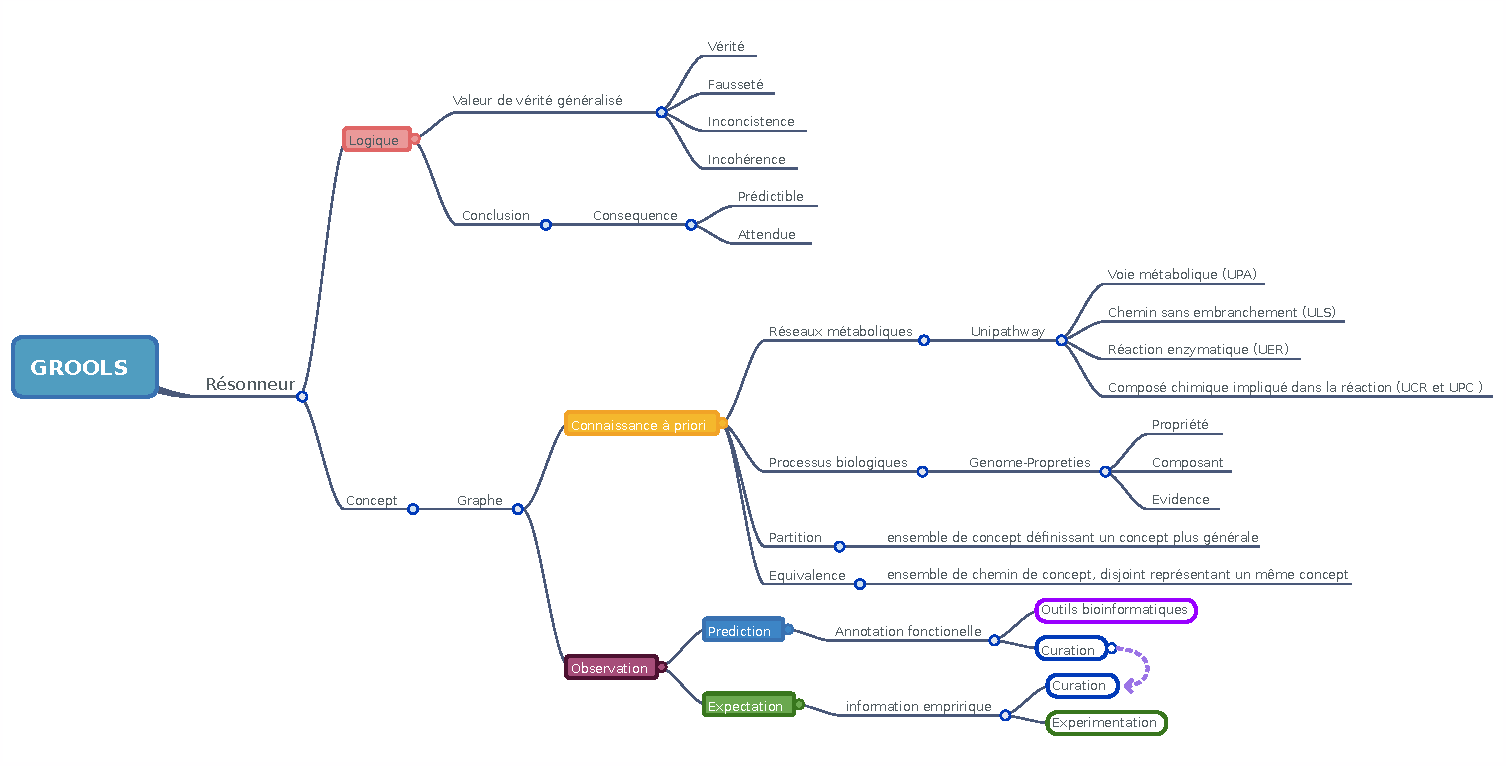
\includegraphics[width=\textwidth]{img/GROOLS_mindmap.pdf}
    \caption{  }
    \label{fig:GROOLS_mindmap}
\end{shadedfigure}

\section{La méthode}
le papier
pdf ici

discussion

\begin{shadedfigure}
    \centering
    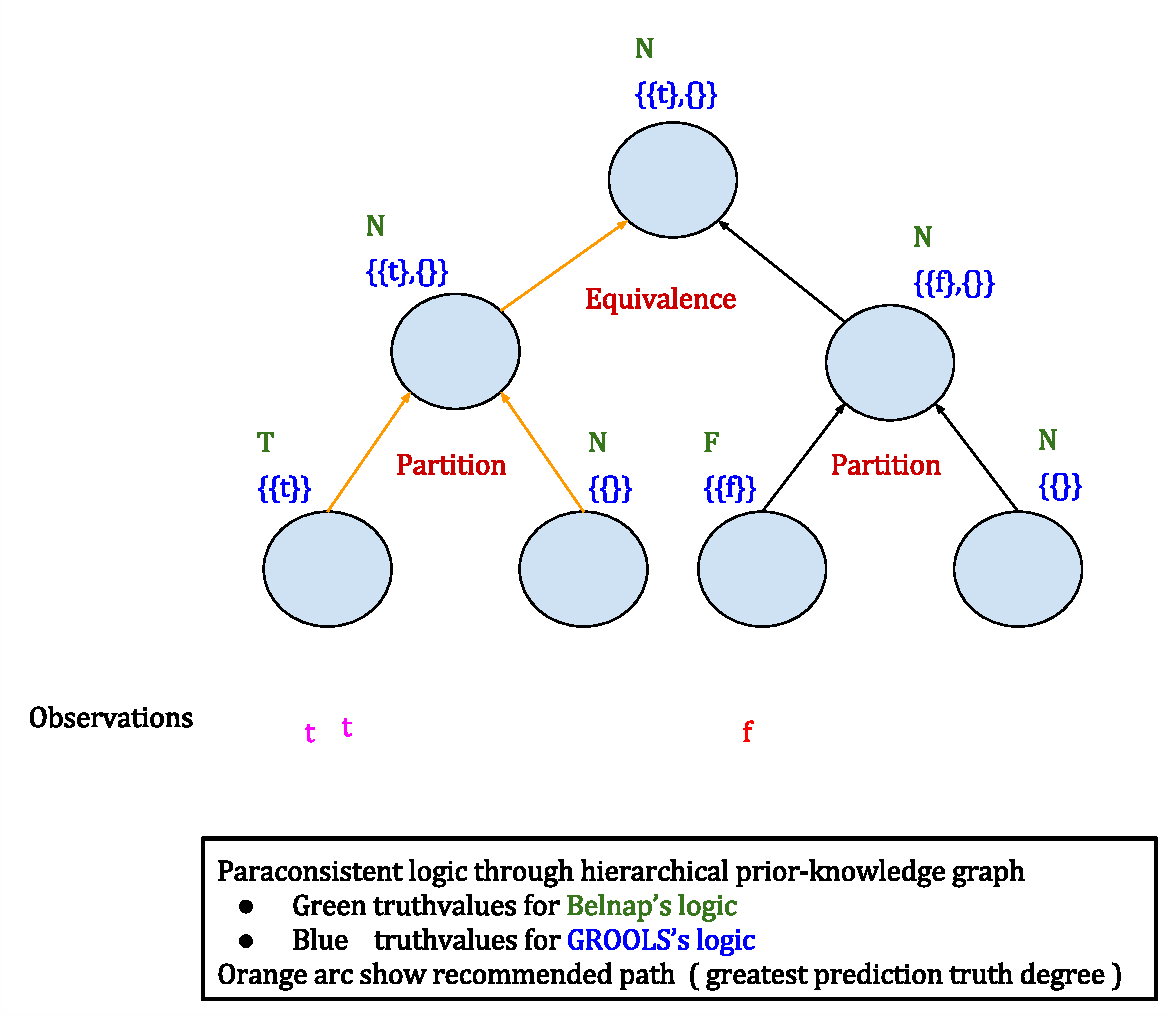
\includegraphics[width=\textwidth]{img/GROOLS_vs_belnap_1.pdf}
    \caption{  }
    \label{fig:grools_belnap_1}
\end{shadedfigure}

\begin{shadedfigure}
    \centering
    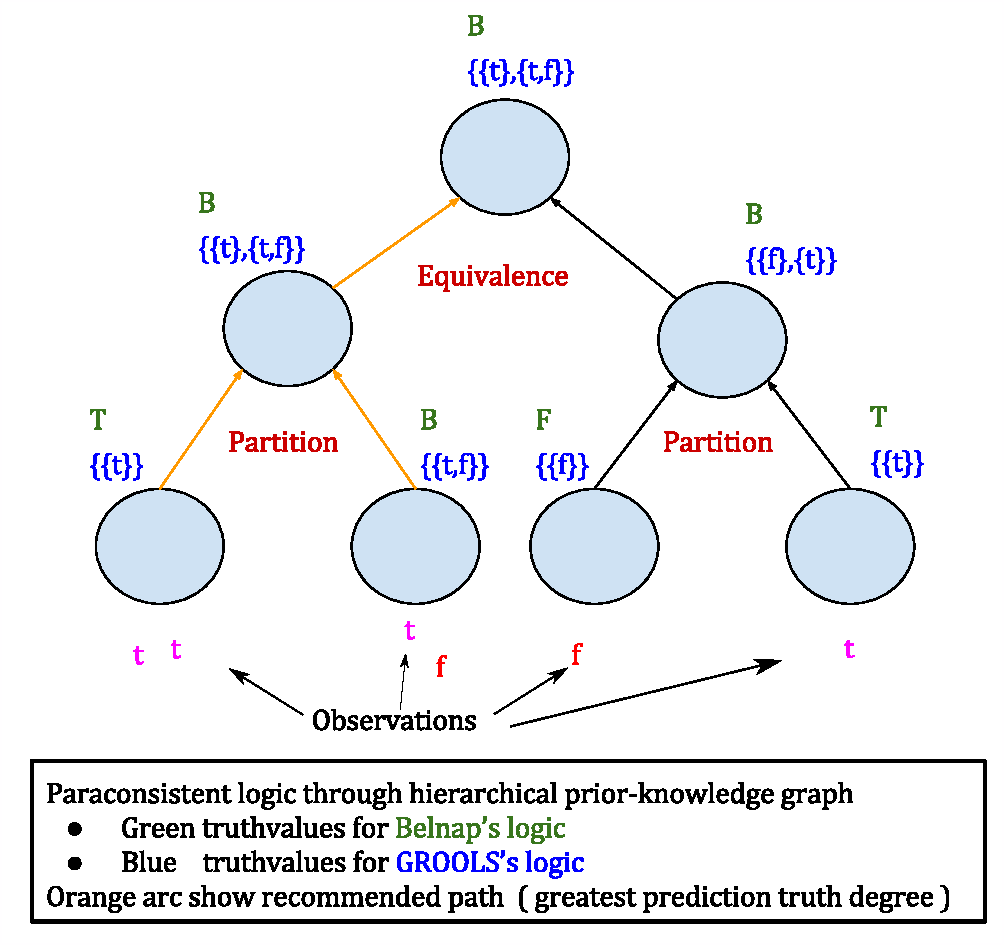
\includegraphics[width=\textwidth]{img/GROOLS_vs_belnap_2.pdf}
    \caption{  }
    \label{fig:grools_belnap_2}
\end{shadedfigure}

\subbibliography
\end{refsegment}